\documentclass{article}
\usepackage[polish]{babel}
\usepackage[T1]{fontenc}
\usepackage[utf8]{inputenc}
\usepackage{graphicx}
\usepackage{float}
\usepackage[bottom=1.5cm, right=1cm, left=1cm, top=1.5cm]{geometry}
\graphicspath{{../pliki}}



\title{%
  Cyberbezpieczeństwo - laboratoria 6 \\
  \large Jednokierunkowe funkcje skrótu \\ Algorytmy wymiany klucza
  }
\author{Patryk Łuszczek 272707}
\date{\today}
\begin{document}
\maketitle
\newpage
\tableofcontents
\newpage

\section{Jednokierunkowe funkcje skrótu}
Do przeprowadzenia ataków zostały wykorzystane 2 pliki tekstowe w wersjach: oryginalna oraz sfałszowana.
\begin{enumerate}
  \item Plik 1
        \begin{enumerate}
          \item \textbf{Oryginalny: } Funkcja haszująca jest ważnym elementem techniki uwierzytelniania wiadomości.
                Otrzymuje ona dane wejściowe o różnej wielkości i wytwarza wartość skrótu o stałej
                wielkości.
                Funkcja haszująca używa funkcji kompresji w sposób powtarzalny, aby
                wygenerować n-bitową wartość wyjściową.
          \item \textbf{Fałszywy: } Funkcja haszująca jest ważnym elementem techniki uwierzytelniania wiadomości.
                Nie otrzymuje ona danych wejściowych o losowej wielkości i wytwarza wartość skrótu o stałej wielkości.
                Funkcja haszująca używa funkcji sinusoidalnej w celu zahaszowania, pliku.
        \end{enumerate}
  \item Plik 2
        \begin{enumerate}
          \item \textbf{Oryginalny: } A hash function is any function that can be used to map data of arbitrary size to fixed-size values, though there are some hash functions that support variable-length output.
                The values returned by a hash function are called hash values, hash codes, hash digests
          \item \textbf{Fałszywy: } A hash function is any function that is not used anymore, though there are some hash functions that may be still viable.
                The values returned by a hash function are used in the medical field to help patients with dementia.
        \end{enumerate}
\end{enumerate}

\subsection{Zadanie}
W celu wykonania zadania wybrano funkcję skrótu SHA-1. Zostały wczytane pliki tekstowe, oryginalny oraz fałszywy. Następnie przeprowadzono atak na z ustaloną długością bitów na 20.
Atak polegał na znalezieniu kolizji dla pierwszych 20-bitów hashu. Oba ataki zostały przeprowadzone pomyślnie.
\begin{table}[H]
  \centering
  \begin{tabular}{|c|c|c|}
    \hline
    \textbf{}         & \textbf{Plik 1}                                   & \textbf{Plik 2}                                   \\ \hline
    \textbf{oryginał} & \textbf{07AEA}044BFCF0EF704D3B150F8FE18F847ECDAF2 & \textbf{A983F}32783100C33E11664A8AF770AF08264BAB1 \\ \hline
    \textbf{fałszywy} & \textbf{07AEA}B227C896E25C1AFB52B4ED431A580F13684 & \textbf{A983F}FE031226F03AD0289F79FA96EA4FC06CF5D \\ \hline
  \end{tabular}
\end{table}
Jak można zauważyć, pierwsz 20 bitów (czyli 5 znaków) hashu są identyczne. W przypadku pierwszego pliku, do obu wersji zostało dopisane 20 pustych znaków, dla drugiego pliku było to 10 i 7 znaków.


\subsection{Zadanie}
\begin{table}[H]
  \caption{Czas ataku dla różnych algorytmów i długości bitów}
  \centering
  \begin{tabular}{|c|c|c|c|c|}
    \hline
    \textbf{Algorytm / bity} & \textbf{20} & \textbf{40} & \textbf{60} & \textbf{80} \\ \hline
    \textbf{MD2}             & 0.01s       & 3h 30min    & 2.7 dni     & 7.7 lat     \\ \hline
    \textbf{MD4}             & 0.01s       & 15s         & 1h          & 43 dni      \\ \hline
    \textbf{MD5}             & 0.01s       & 17s         & 1h          & 55 dni      \\ \hline
    \textbf{SHA-1}           & 0.02s       & 27s         & 53m         & 66dni       \\ \hline
    \textbf{RIPEMD-160}      & 0.03s       & 34s         & 2h 25m      & 180dni      \\ \hline
  \end{tabular}
\end{table}

\subsection{Jak rośnie czas realizacji ataku wraz ze wzrostem wartości parametru opisującego długość ustalonego ciągu bitów?}
Czas rezlizacji ataku jest ściśle powiązany z parametrem opisującym długość ciągu bitów. Wraz ze wzrostem tego parametru,
czas realizacji wzrasta wykładniczo. Dla długości 20bitów atak został przeprowadzony natychnmiastowo, natomiast dla długości 80 bitową, przewidywany czas realizacji wynosi kilkadziesiąt dni.
\subsection{Czy wybór funkcji skrótu ma wpływ na czas realizacji zadania poszukiwania kolizji?}
Jak można zauważyc, czas realizacji ataku jest ściśle powiązany nie tylko z liczbą bitów, ale również z wybraną funkcją skrótu. Dla małej wartości bitów, wyniki dla wszystkich funkcji były praktycznie takie same.
Dla 40-bitów, czas poszukiwania był bardzo przybiliżony dla wszystkich funkcji oprócz algorytmu MD2, który był znacznie wolniejszy od pozostałych. Dla kolejnych długości bitów, czas dla każdego z algorytmu
rósł, lecz nie jednakowo. Najwolniej trwało poszukiwanie kolizji dla MD2, a najszybciej dla MD4. Problem z długim czasem poszukiwania kolizji dla MD2, może być związany z faktem, że jest to przestarzał algorytm,
który nie jest zoptymalizowany pod kątem współczesnych procesorów - został stworzony z myślą o 8-bitowych komputerach.
% te nastepne do wlasnego zastanowienia/ wyszukania
\subsection{Na czym polega przewaga modyfikowania dwóch dokumentów nad poszukiwaniem kolizji przy modyfikacji tylko jendego dokumentu?}
Kiedy modyfikowany jest tylko jeden dokument, musi on zostać dopasowany do hashu drugiego dokumentu, a tkaich kombinacji jest \(2^{n}\), gdzie n oznacza długość hashu. Oznacza to, że prawdopobieństwo znalezienia kolizji wynosi
\(\frac{1}{2^{n}}\), czyli jest ono niezwykle niskie. Jeśli modyfikowane są oba dokumenty, prawdopobieństwo to wzrasta, ponieważ nie szukamy dopasowania do jednego konkretnego hasha, tylko szukamy takiej modyfikacji dokumentów, która da nam jednako hash - nieważne jaki.
Dzięki modyfikowaniu obu dokumentów rośnie tam liczba potencjalnych dopasowań, która przy wykorzystaniu ataku urodzinowego daje szanse sukcesu \(\frac{1}{2^{n/2}}\)

\subsection{Czy w świetle uzyskanych wyników możemy ufać funkcjom skrótu?}
Mimo, że eksperyment został przeprowadzony tylko dla 60 bitów, można stwierdzić, że funkcje skrótu mają swoje słabości i ograniczenia. Dla wartości bitów podanych w eksperymencie
udało się znaleźć kolizję, co wskazuje na to, że przepadane funkcje skrótu nie śa idealne. Dodatkowo funkcje takie jak MD5 oraz SHA-1 obecnie są uważane za niebezpiecznie i nie są zalecane.
Więc w celu zwiększenia bezpieczeńswa, zaleca się korzystanie z silniejszych funkcji, takichj jak np. SHA-256 lub SHA-3.
\subsection{Jakiego typu problemy zostały zidentyfikowane dla popularnych funkcji skrótu (MD5, SHA)?}
W przypadku obu tych funkcji, zostało udowodnione, że śa ole podatne na kolizje, i że nie powinny być używane
do zastosowań kryptograficznych (podpisy cyfrowe, certyfikaty, itp.). Dla MD5, zostało to pokazane już w 2004 roku. W przypadku SHA-1, w 2017 roku został
zaprezentowany pierwszy publiczny atak kolizji nazwany "SHAttered". Zostały pokazane dwa całkiem niepodobne pliki PDF, a sam atak miał być 100 000 razy szybszy
niż atak brute-force z wykorzystaniem ataku urodzinowego.

\section{Wymiana klucza kryptograficznego}
tutaj screeny z podpisem ktory to klient

\begin{itemize}
  \item Generowanie wspólnego klucza DH:
        \begin{figure}[H]
          \centering
          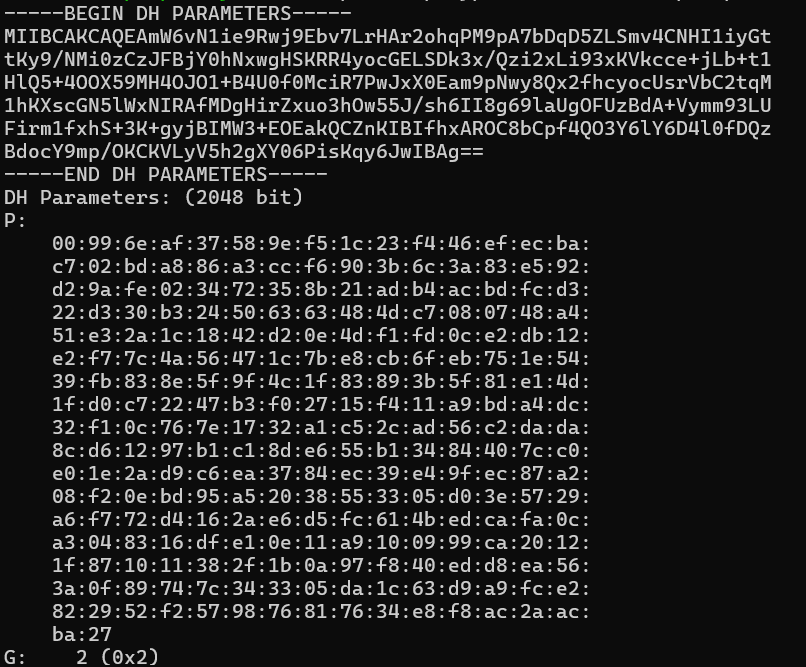
\includegraphics[width=0.5\textwidth]{klucz_wspolny.png}
        \end{figure}
  \item  Klucz dla klienta 1:
        \begin{figure}[H]
          \centering
          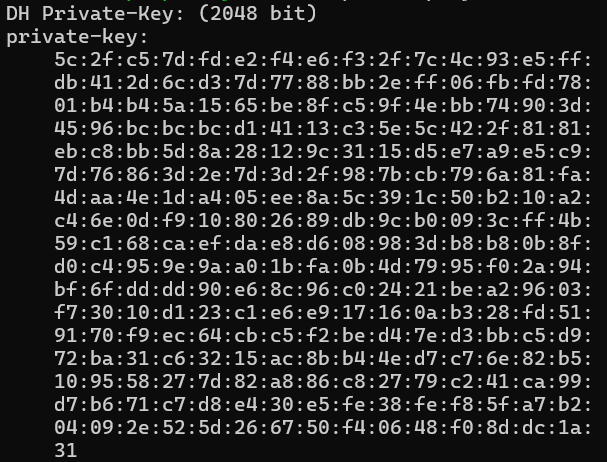
\includegraphics[width=0.5\textwidth]{client1_private_key.png}
        \end{figure}
  \item Klucz dla klienta 2:
        \begin{figure}[H]
          \centering
          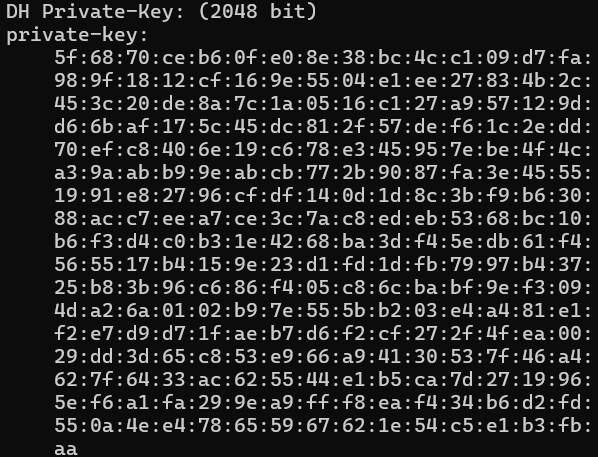
\includegraphics[width=0.5\textwidth]{client2_private_key.png}
        \end{figure}
  \item Klucz tajny dla obu klientów jest jednakowy, komenda cmp nie zwróciła żadnego wyniku, który wskazywałby na różnice między nimi
  \item Secret key 1
        \begin{figure}[H]
          \centering
          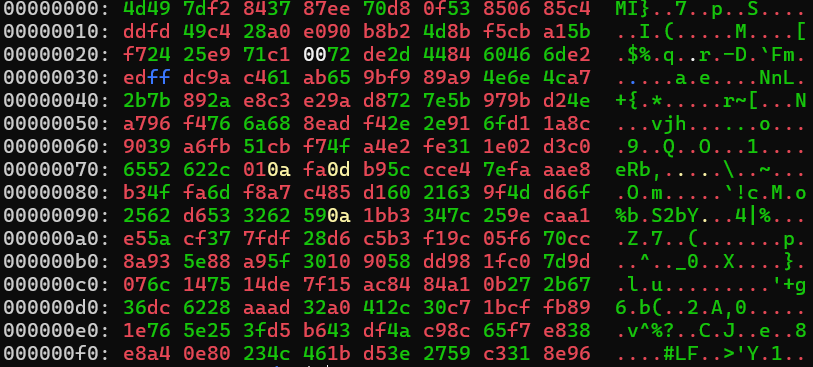
\includegraphics[width=0.5\textwidth]{secret_key1.png}
        \end{figure}
  \item Secret key 2
        \begin{figure}[H]
          \centering
          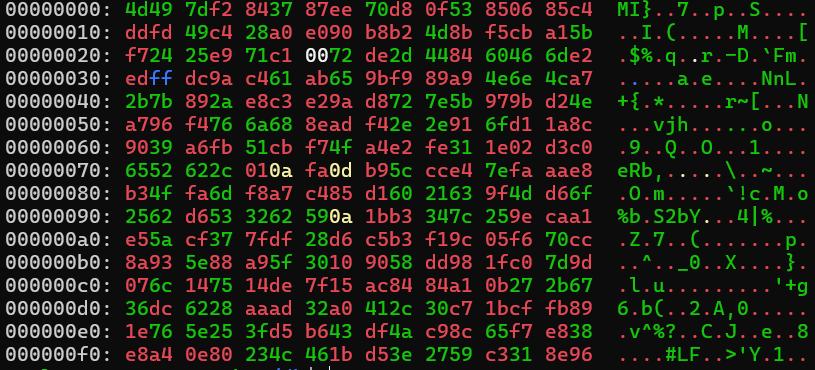
\includegraphics[width=0.5\textwidth]{secret_key2.png}
        \end{figure}
\end{itemize}

\subsection{Który sposób wymiany kluczy gwarantuje większe bezpieczeństwo i dlaczego (RSA vs DH)}
Oba sposoby wymiany kluczy mają swoje wady i zalety. Dla przykładu DH nie zapewnia możliwości autoryzacji autorów wiadomości,
co jest podstawą RSA. W związku z tym, nie może być wykorzystywany przy podpisie elektronicznym, gdyż może zostać przerobiony, a odbiorca nie będzie mógł zweryfikować
czy otrzymana wiadomość jest poprawna (man-in-the-middle). Jednakże, RSA nie zapewnia "perfect forward secrecy", które jest obecne w DH.
Oznacza to, że jeśli osoba trzecia pozna klucz używany w RSA będzie mogła odszyfrować wcześniejsze wiadomości, nie ma to natomiast miejsca w przypadku DH.
Tak więc, każdy sposób ma swoje wady i zalety, powinny zostać używane do przeznazonych dla siebie celów.

\subsection{Jakie jest ryzyko dla podmiotów korzystających z protokołu wymiany kluczy DH?}
Jednym z zasadnicych zagrożen wynikających z protokołu wymiany kluczy DH jest podatność na atak typu Man-In-The-Middle. Wiąże się to z brakiem
mechanizmu autoryzacji, który pozwalałbym na weryfikację wiadomości otrzymanych od drugiej strony. Atakujący może dowolnie manipulować wiadomościami bez wiedzy żadnej ze stron.
Podczas takiego ataku, atakujący może uzyskać dostęp do do wiadomości, poprzez zmianę transmitowanego klucza na własny. W celu zabezbieczenia się przed tego typu atakiem,
zaleca się wykorzystanie pewnej formy uwierzytelnienia, np. protokołu PAKE (Password Authentification Key Agreement).
\subsection{Jakie są inne metody określania wspólnego klucza krypotgraficznego (oprócz DH)}
Oprócz DH oraz RSA, można spotkać się jeszcze z wieloma innymi podejściami. Jednym z nich jest wykorzystanie QKD (quantum key distribution), który wykorzystuje podstawowe zasady mechaniki kwantowej. Obie strony
tworzą losowy tajny klucz współdzielony, który jest używany do szyfrowania i deszyfrowania. Zaletą tego podejścia, jest możiwość wykrycia osób trzecich próbujących podsłuchać transmisję. Innym sposobem jest wkorzystanie sieci zaufania, która jest zdecentrelizowaną
metodą uwierzytelniania. Każdy uczesnij sieci "podpisuje" klucze osób, które osobiście zweryfikował. Kolejnym sposobem może być PKA (password authenticated key agreement), który wykorzystuje znajomość hasła przez jedną lub więcej stron.
\subsection{Który element protokołu DH nie jest przesyłany między klientami? Jak to wpływa na kwestie bezpieczeństwa?}
W protokole DH nie jest przesyłany klucz prywatny, ustalany indywidualnie dla każdej ze stron. Dzięki kluczowi prywatnemu, strony mogą ustalić wspólny klucz, który jest obecnie niemożliwy do odszyfrowania,
jeśli poszczególne parametry są wystarczająco skomplikowane.
\subsection{Sprawdź czy w ostatnim punkcie udał się ustalić ten sam klucz dla obu klientów. Uwzlgędnij w raporcie treść uzgodniionego tajnego klucza.}
W wyniku eksperymentu udało się uzyskać ten sam klucz dla obu klientów, jego treść została zamieszczona we wcześniejszej części raportu.
\end{document}